\chapter{Cài đặt và triển khai}

\section{Công nghệ sử dụng}
\begin{itemize}
  \item \textbf{Frontend}: Next.js (App Router), React, Tailwind CSS.
  \item \textbf{Crypto client}: Web Crypto API (AES‑GCM, PBKDF2), Ethers.js (ký thông điệp).
  \item \textbf{Backend}: Next.js API routes, JWT (HS256), CSRF double‑submit cookie.
  \item \textbf{Lưu trữ}: Ciphertext local theo CID (SHA‑256 demo), metadata trong SQLite.
\end{itemize}

\section{Cấu trúc dữ liệu chính}
\begin{itemize}
  \item \texttt{files}: id, owner\_address, title, description, cid, name, mime, size\_bytes, iv, (salt, iv\_wrap, wrapped\_key | raw\_key\_base64), created\_at.
  \item \texttt{tokens}: token, file\_id, issued\_to\_address, expires\_at, revoked, created\_at.
\end{itemize}

\section{Các API tiêu biểu}
\begin{itemize}
  \item \texttt{POST /api/auth/start}: phát nonce; \texttt{POST /api/auth/verify}: xác minh chữ ký, set JWT.
  \item \texttt{POST /api/storage/upload}: nhận ciphertext (octet‑stream), trả CID.
  \item \texttt{POST /api/files}: lưu metadata (IV, CID, key info), phát token TTL.
  \item \texttt{POST /api/tokens/validate}: trả metadata theo token; \texttt{POST /api/tokens/revoke}: thu hồi.
\end{itemize}

\section{UI Screenshots}
\begin{figure}[H]
  \centering
  \begin{subfigure}{0.48\textwidth}
    \centering
    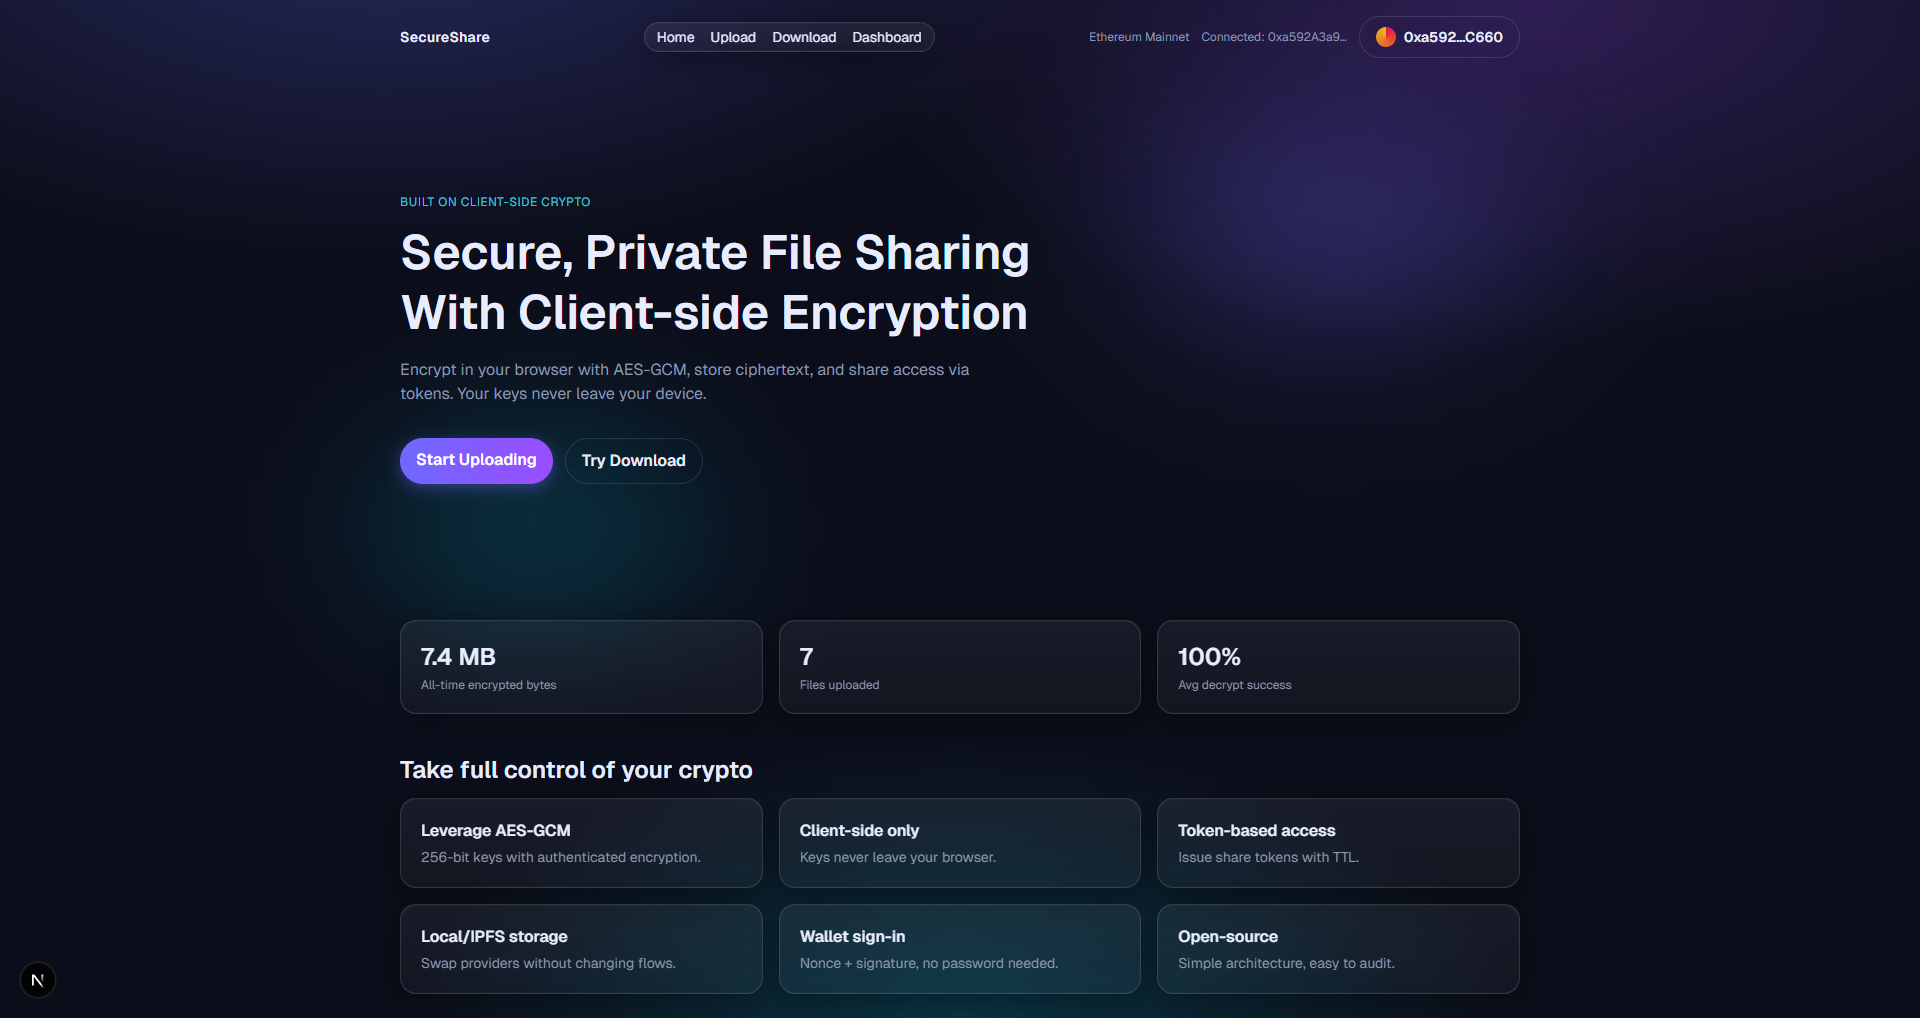
\includegraphics[width=\linewidth]{ui-home.png}
    \caption{Home Page with Hero Section}
  \end{subfigure}\hfill
  \begin{subfigure}{0.48\textwidth}
    \centering
    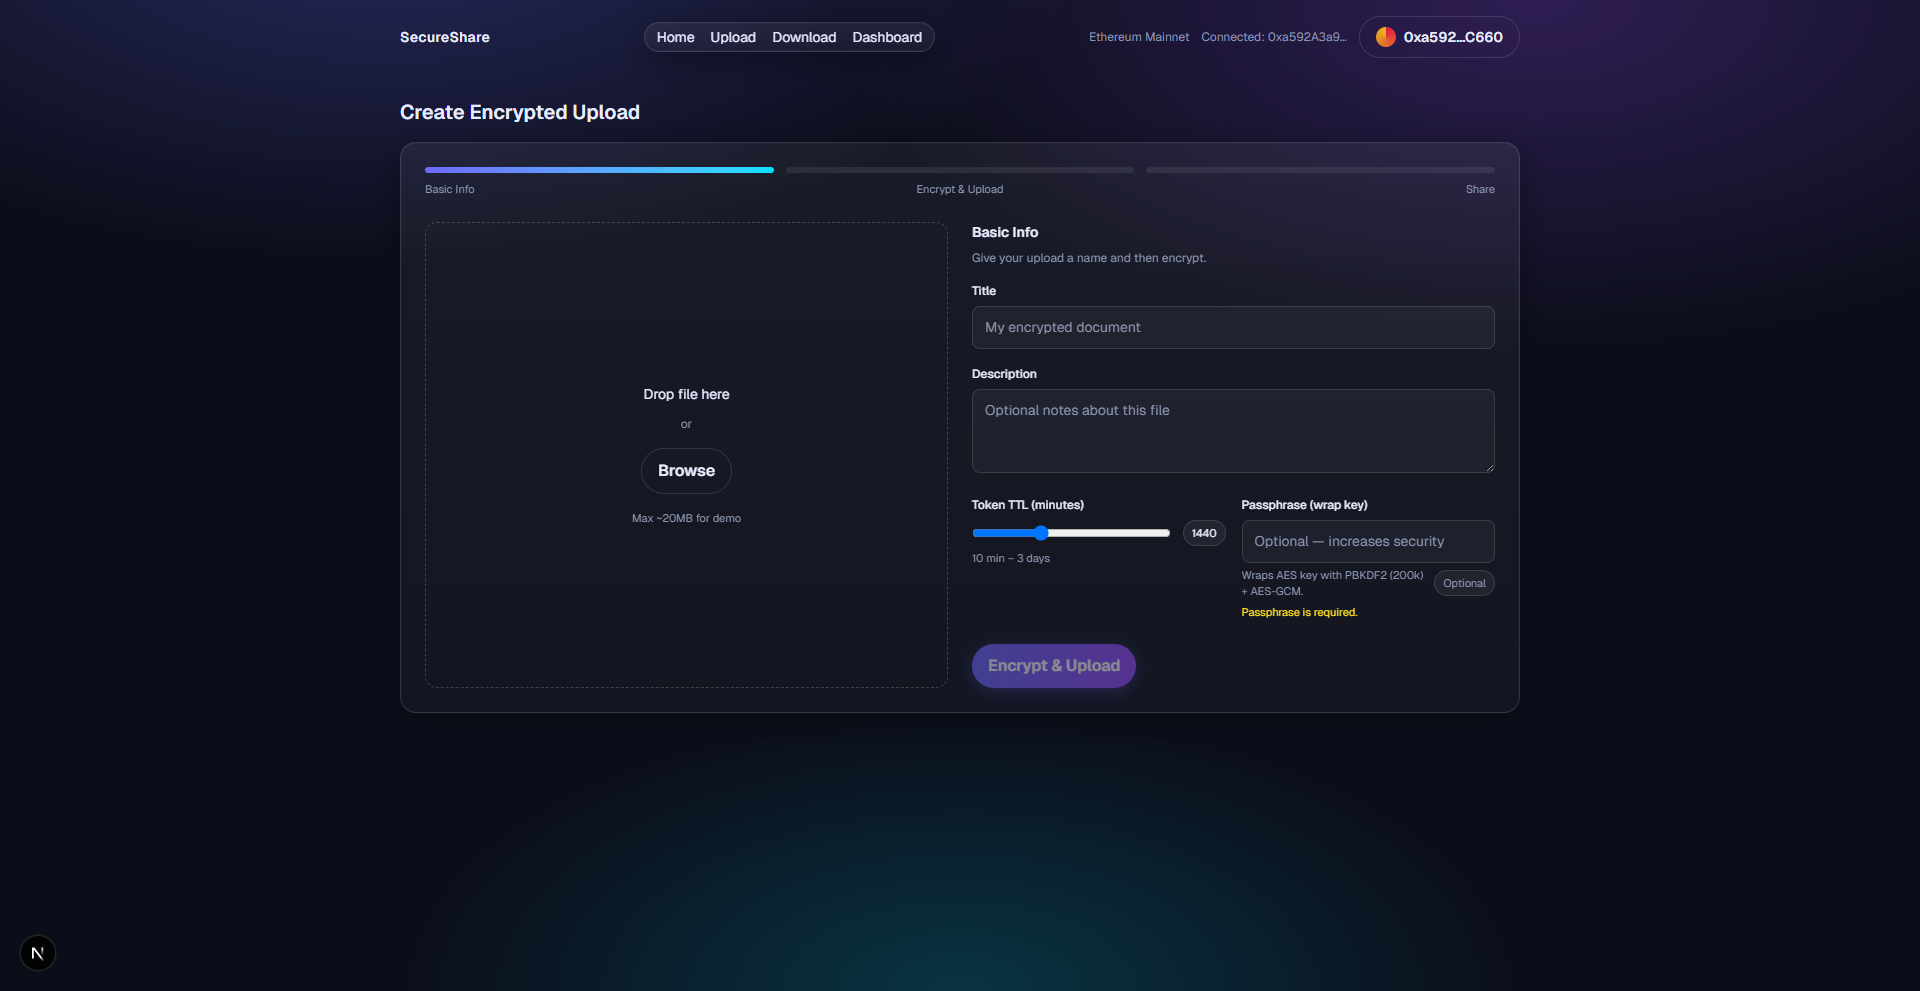
\includegraphics[width=\linewidth]{ui-upload.png}
    \caption{Upload Page with Encryption Wizard}
  \end{subfigure}
  \caption{Application Interface - Part 1}
\end{figure}

\begin{figure}[H]
  \centering
  \begin{subfigure}{0.48\textwidth}
    \centering
    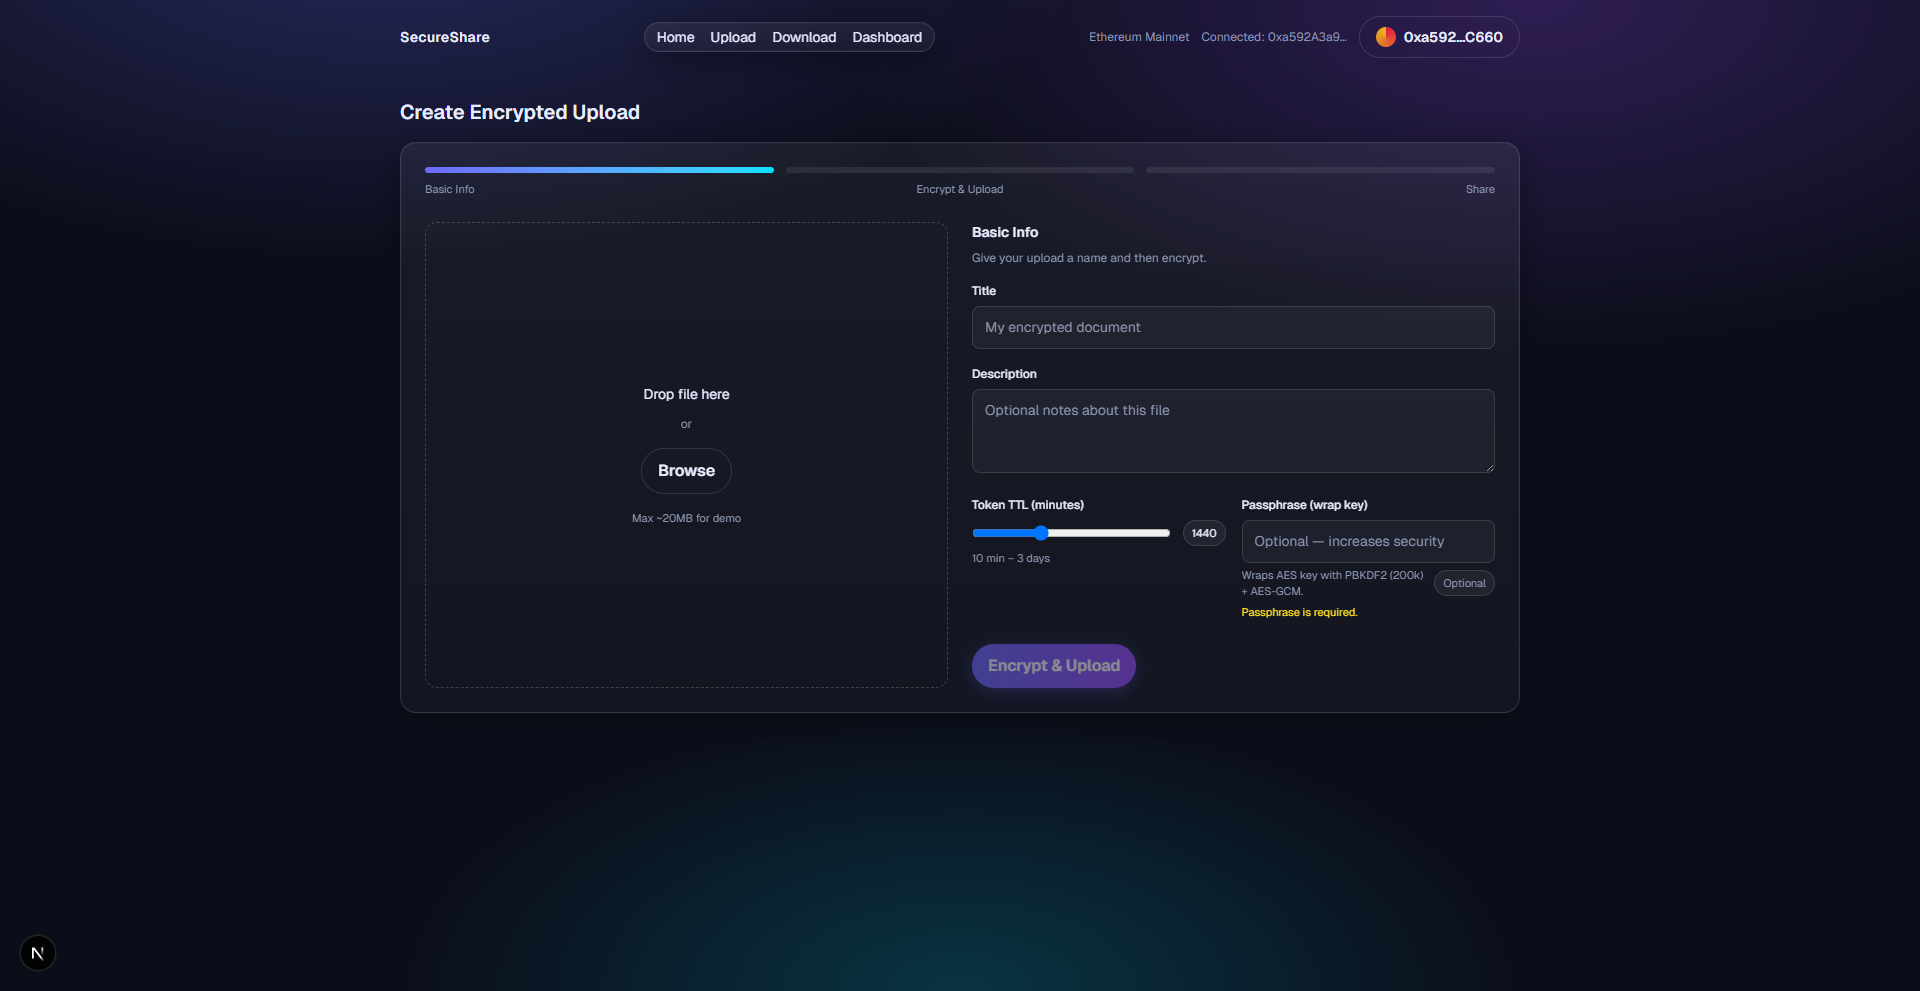
\includegraphics[width=\linewidth]{ui-download.png}
    \caption{Download \& Decrypt Page}
  \end{subfigure}\hfill
  \begin{subfigure}{0.48\textwidth}
    \centering
    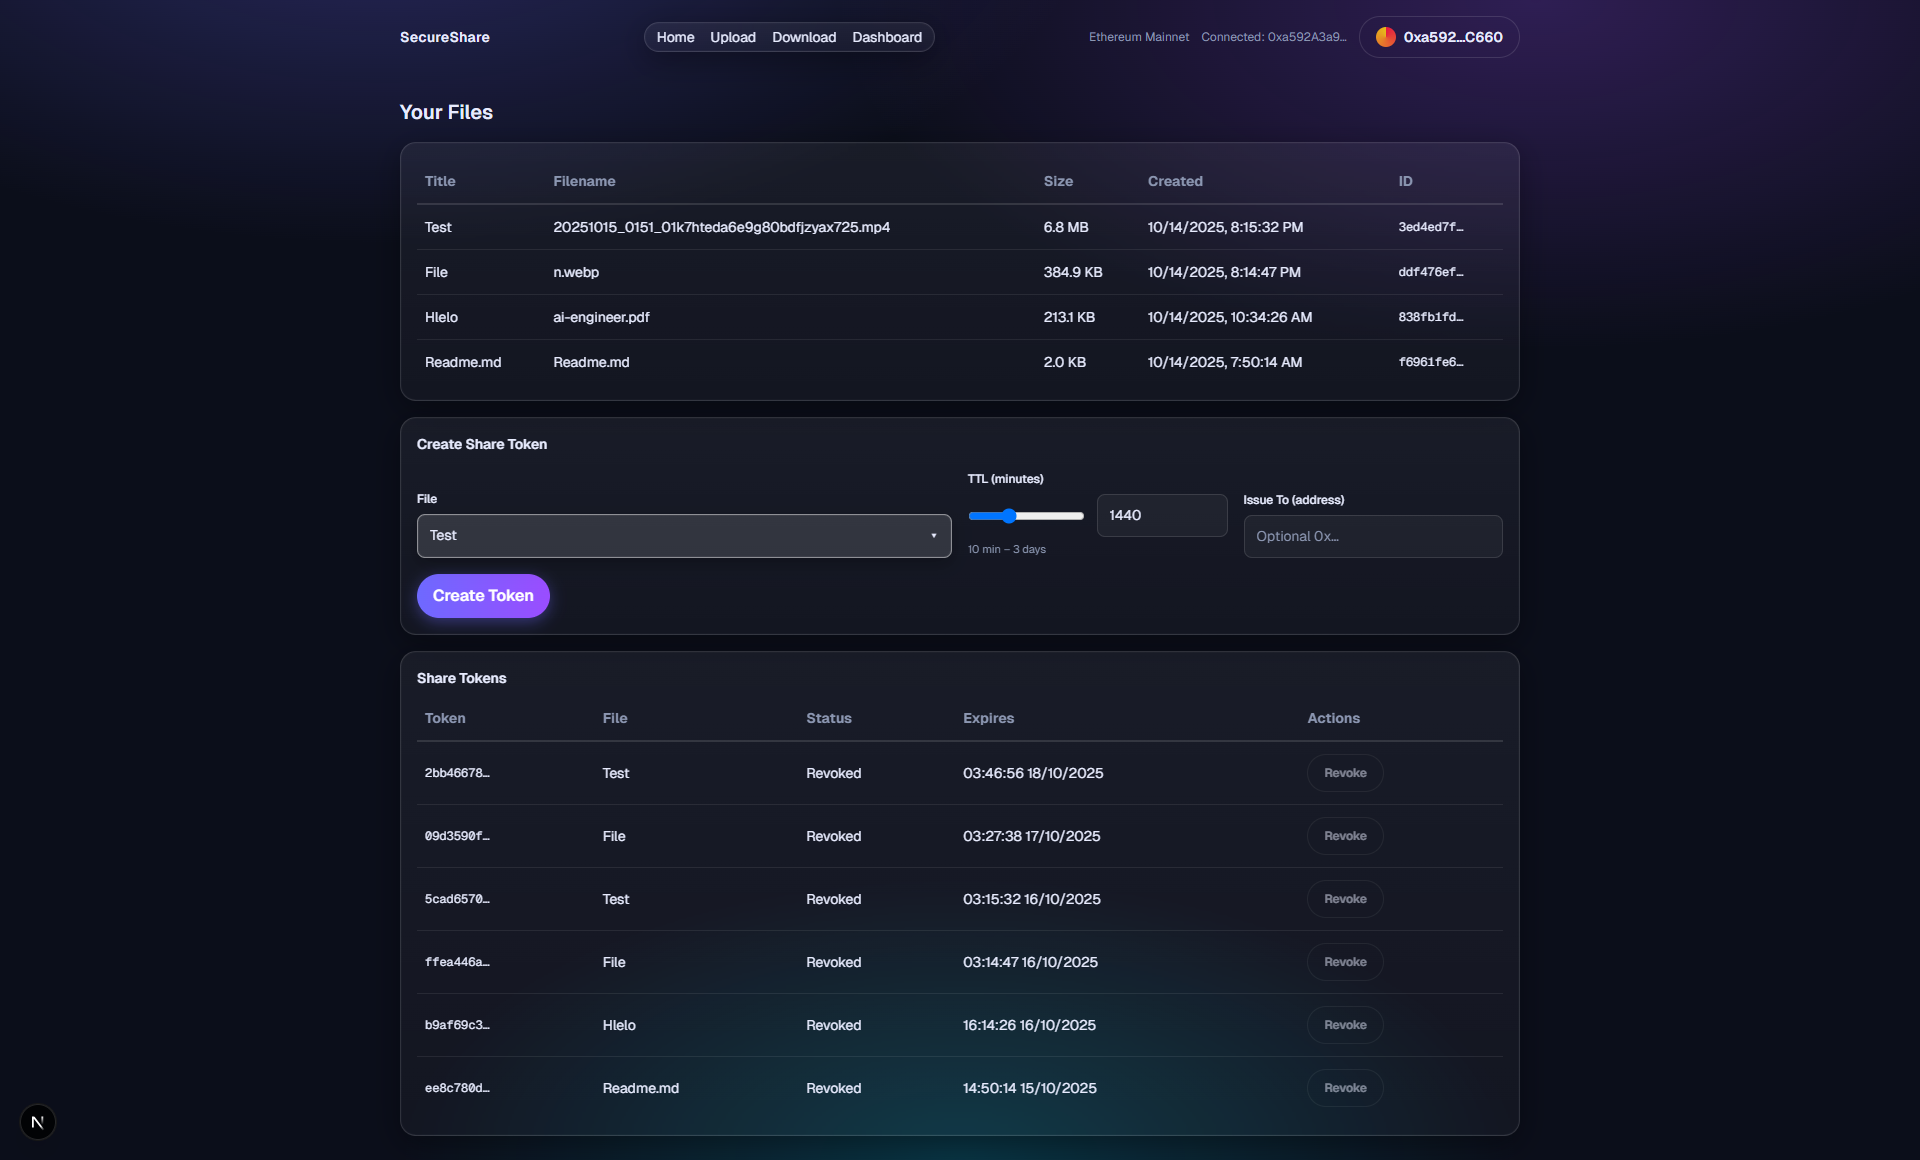
\includegraphics[width=\linewidth]{ui-dashboard.png}
    \caption{Dashboard with File Management}
  \end{subfigure}
  \caption{Application Interface - Part 2}
\end{figure}

\section{Installation \& Setup}
\subsection*{Prerequisites}
\begin{itemize}
  \item Node.js v18 or higher
  \item npm v9 or higher
  \item MetaMask browser extension (for wallet integration)
\end{itemize}

\subsection*{Installation Steps}
\begin{enumerate}
  \item Clone or extract the project repository
  \item Navigate to the project root directory
  \item Run \texttt{npm install} to install dependencies
  \item Create \texttt{.env.local} file with required environment variables
  \item Run \texttt{npm run dev} to start the development server
  \item Open \texttt{http://localhost:3000} in your browser
\end{enumerate}

\section{User Guide}
\subsection*{1. Connecting Your Wallet}
To use the application, connect your Ethereum wallet (MetaMask):
\begin{enumerate}
  \item Click the \textbf{``Connect Wallet''} button in the top-right corner
  \item MetaMask will open; select your account and approve the connection
  \item Sign the authentication message (nonce) to verify ownership
  \item Your wallet address will appear in the header
\end{enumerate}

\subsection*{2. Uploading and Encrypting a File}
To upload a file with encryption:
\begin{enumerate}
  \item Navigate to the \textbf{Upload} page
  \item Drag and drop a file or click \textbf{Browse} to select one
  \item Enter a \textbf{Title} and optional \textbf{Description}
  \item (Optional) Enter a \textbf{Passphrase} to wrap the AES key (recommended for production)
  \item Adjust \textbf{Token TTL} (time-to-live) from 10 minutes to 3 days
  \item Click \textbf{Encrypt \& Upload}
  \item The file is encrypted client-side using AES-256-GCM; only ciphertext is sent to the server
  \item A share token is generated and displayed
\end{enumerate}

\subsection*{3. Sharing the File}
After uploading:
\begin{enumerate}
  \item Copy the \textbf{Share Token} or \textbf{Download Link}
  \item Send the token/link to the recipient via any communication channel
  \item The recipient can use the token to download and decrypt the file
  \item Tokens can be revoked at any time from the Dashboard
\end{enumerate}

\subsection*{4. Downloading and Decrypting a File}
To decrypt and download a shared file:
\begin{enumerate}
  \item Navigate to the \textbf{Download} page (or use the share link directly)
  \item Paste the \textbf{Token} into the input field
  \item Click \textbf{Validate} to check token validity and retrieve file metadata
  \item If the file was wrapped with a passphrase, enter it
  \item Click \textbf{Download \& Decrypt} to download the decrypted file
  \item The decryption happens entirely in your browser; the server never sees the decrypted content
\end{enumerate}

\subsection*{5. Managing Files and Tokens}
On the \textbf{Dashboard}:
\begin{itemize}
  \item View all files you have uploaded (owner only)
  \item See file details: name, size, upload date
  \item Issue new tokens for any of your files
  \item Revoke existing tokens to immediately disable access
  \item Manage token TTL and optionally restrict tokens to specific addresses
\end{itemize}

